\documentclass{article}
\usepackage[utf8]{inputenc}
\usepackage[margin=1.2in]{geometry}
\usepackage{hyperref}

\usepackage{tikz}
\usetikzlibrary{positioning}

\usepackage{natbib}
\usepackage{graphicx}
\usepackage{amsmath}

\title{\vspace{-2 cm}Universidade Federal de Ouro Preto \\ BCC 325 - Inteligência Artificial \\ Busca em Espaço de Estados}
\author{Prof. Rodrigo Silva}
\date{}


\begin{document}

\maketitle

\section{Leitura}

\begin{itemize}
    \item Ler o capítulo 3 do Livro\textit{ Artificial Intelligence: Foundations of Computational Agents,  2nd Edition} disponível em \textit{https://artint.info/}
\end{itemize}

\section{Questões teóricas}

\begin{enumerate}
    
    \item Quais algoritmos de busca em espaço de estados você utilizaria para encontrar o caminho de menor custo entre um estado inicial e um estado final (ou meta)? Compare os algoritmos selecionados em termos de custo computacional (tempo de execução e espaço de memória) e apresente vantagens e desvantagens na utilização de cada um dos métodos. 

    \item  O algoritmo \textit{Iterative Deepening} (Aprofundamento Iterativo) aplica uma busca em profundidade impondo um limite na profundidade máxima a ser pesquisada. Este limite é incrementado de um em um até que um estado alvo seja encontrado ou até que a árvore toda seja pesquisada. Explique como esta estratégia elimina desvantagens e combina vantagens de ambos, Busca em largura e Busca em Profundidade.
    
    
    \item Selecione a opção correta para cada célula da tabela. $h(n)$ é o valor da função heurística do nó $n$. $c(S,n)$ é o custo do caminho de um nó $S$ até o nó $n$.
    
    \begin{center}
        \begin{tabular}{|l|c|c|c|}
        \hline
        Estratégia            & Seleção da fronteira & Caminho Encontrado & Custo em Espaço \\
        \hline
        Busca em Largura      &     &   &   \\
        \hline
        Busca em Profundidade &     & (g)  &   \\
        \hline
        Guloso                &     &   &   \\
        \hline
        Menor Caminho Primeiro& (b) &   &   \\
        \hline
        $A^*$                 &     &   &   \\
        \hline
        Branch and Bound      &     &   &   \\
        \hline
    \end{tabular}
    \end{center}
    
    \begin{enumerate}
        \item Menor $h(n)$
        \item Menor $c(S,n)$
        \item Menor $h(n) + c(S,n)$
        \item Primeiro caminho adicionado 
        \item Último caminho adicionado 
        \item Menor número de arcos
        \item Indefinido
        \item Menor custo
        \item Linear 
        \item Exponencial
    \end{enumerate}
    
    \item Para o que serve função heurística em alguns algoritmos e busca? 
    
    \item Como funciona o algoritmo de poda de ciclos?
    
    \item Como funciona o algoritmo de poda de múltiplos caminhos?
    
    \item Considere o grafo abaixo onde o 1 representa o estado inicial e o nó 11 é o objetivo. O custo de cada aresta é a diferença entre os valores do nó filho de do nó pai.
    
    \begin{figure}[!ht]
        \centering
        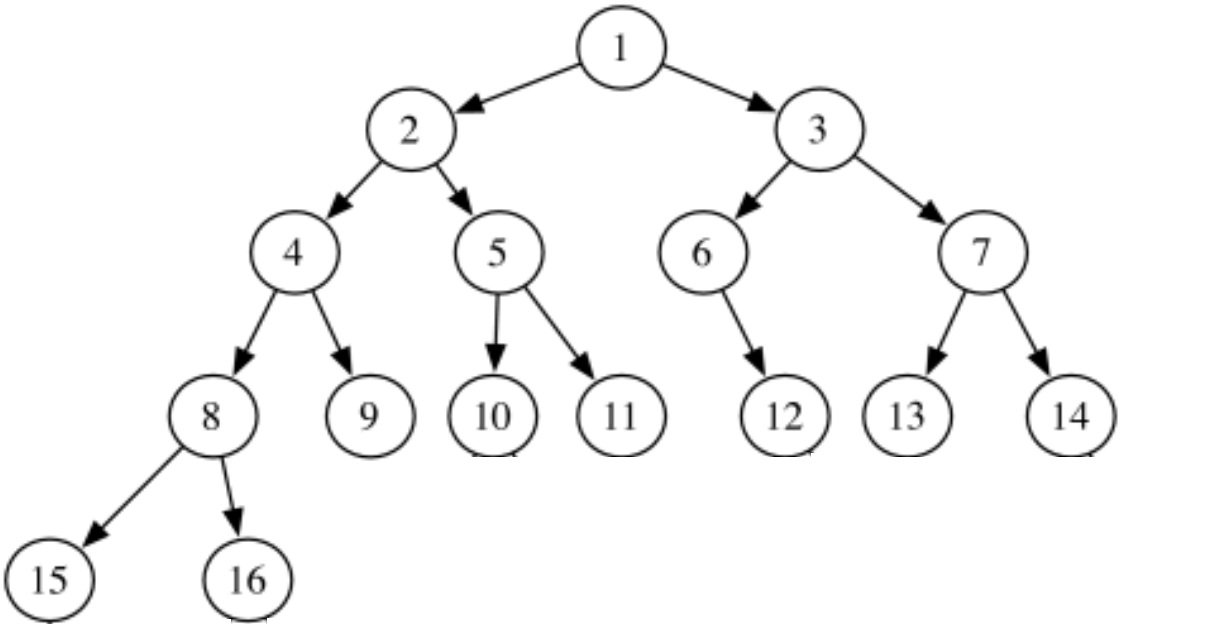
\includegraphics[width=0.5\textwidth]{graph.PNG} \label{fig:my_label}
    \end{figure}
    
    Apresente o estado da fronteira a cada iteração para os seguintes métodos.
    
    \begin{enumerate}
        \item Busca em largura 
        \item Busca em profundidade
        \item Menor custo primeiro
    \end{enumerate}
    
\end{enumerate}

\section{Atividade Prática}

Nesta atividade você deve desenvolver um sistema agente/ambiente em que o agente explora um campo com obstáculos (ambiente). Dada um posição inicial e uma posição final, o agente deve encontrar o caminho de uma até a outra, desviando dos obstáculos, utilizando os seguinte algoritmos de busca:

\begin{enumerate}
    \item Busca em largura
    \item Busca em profundidade
    \item Algoritmo guloso
    \item Menor custo primeiro
    \item A*
    \item Branch-and-bound
\end{enumerate}

Você deve implementar tanto o agente e o ambiente.



% Na leitura recomendada você deve ter lido que agentes são entidades que interagem com um ambiente. Nesta atividade você deve implementar agentes que encontram o caminho de uma posição inicial até uma posição alvo desviando de objetos. 

% Visite o repositório \url{https://github.com/rcpsilva/BCC740\_ArtificialIntelligence}, que contem o código base para esta atividade e leia atentamente o README.

% O arquivo \textit{Room.py} contém a classe \texttt{Room} que implementa um \texttt{Environment} que representa uma sala com obstáculos. Atributos importantes desta classe são:

% \begin{itemize}
%     \item \texttt{room}: É uma matriz que contém 0 nas posições livres e 0 nas posições com obstáculos.
%     \item \texttt{initial\_positon}: Posição inicial do agente na sala.
%     \item \texttt{target}: Posição em que o agente deve chegar.
% \end{itemize}

% O método de classe \texttt{initial\_percepts()} retorna:

% \begin{itemize}
%     \item \texttt{current\_position}: com a posição inicial do agente.
%     \item \texttt{target}: com a posição em que o agente deve chegar.
%     \item \texttt{neighboors} com as posições vizinhas livres. 
% \end{itemize}

% O método de classe \texttt{signal(action)} retorna:

% \begin{itemize}
%     \item \texttt{current\_position}: com a posição atual do agente.
%     \item \texttt{target}: com a posição em que o agente deve chegar.(Obs: Esta opção está aqui para modelar a possibilidade de mudança de objetivo durante a execução.)
%     \item \texttt{neighboors} com as posições vizinhas livres. 
% \end{itemize}

% Uma \texttt{action} é, da lista de vizinhos livres, a posição para onde o agente quer se mover. 

% Veja o exemplo ilustrado na figura \ref{fig:room}.

% \begin{figure}[!ht]
%     \centering
%     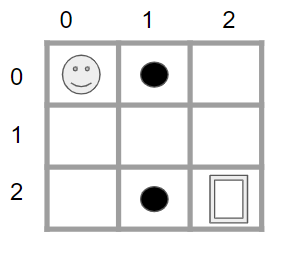
\includegraphics[width=0.4\textwidth]{room.PNG}
%     \caption{Ilustração da classe \texttt{Room}}
%     \label{fig:room}
% \end{figure}

% Para o exemplo mostrado na figura \ref{fig:room} teríamos:
%     \[
%         \texttt{room} = \begin{bmatrix}
%             0 & 1 & 0\\ 
%             0 & 0 & 0\\ 
%             0 & 1 & 0
%         \end{bmatrix}
%     \]
    
%     \[
%         \texttt{begin} = [0,0]
%     \]
    
%     \[
%         \texttt{target} = [2,2]
%     \]
    
%     \[
%         \texttt{current\_position} = [0,0]
%     \]
    
%     \[
%         \texttt{target} = [2,2]
%     \]
    
%     \[
%         \texttt{neighboors} = [[1,0],[1,1]]
%     \]

% o arquivo \textit{path\_finder\_agents.py} contém a implementação do \texttt{RandAgent}. Em cada posição, este agente escolhe um vizinho livre aleatoriamente para visitar. Ele para quando chega à posição alvo. Este agente pode ser usando como base para a implementação de outros agentes.

% Dadas estas informações, faça:

% \begin{enumerate}
%     \item Clone repositório \url{https://github.com/rcpsilva/BCC740\_ArtificialIntelligence}, leia atentamente o README e trabalhe a partir dele.
%     \item Execute o arquivo \textit{path\_finder\_simulation.py} para ver como o RandAgent se comporta.
%     \item No arquivo \textit{path\_finder\_agents.py}, implemente a classe \texttt{BFSAgent} que representa um agente que encontra a posição alvo fazendo uma busca em largura.
%     \item No arquivo \textit{path\_finder\_agents.py}, implemente a classe \texttt{DFSAgent} que representa um agente que encontra a posição alvo fazendo uma busca em profundidade.
%     \item No arquivo \textit{path\_finder\_agents.py}, implemente a classe \texttt{GreedyAgent} que representa um agente que encontra a posição alvo utilizando o algoritmo guloso.
%     \item No arquivo \textit{path\_finder\_agents.py}, implemente a classe \texttt{AStarAgent} que representa um agente que encontra a posição alvo utilizando o algoritmo A$^*$.
% \end{enumerate}

% Observações:
% \begin{itemize}
%     \item Todos os agentes implementados devem fazer poda de ciclos e poda de múltiplos caminhos.
%     \item Os agentes devem implementar a interface \texttt{Agent} definida no arquivo \textit{definitions.py}. 
%     \item Métodos auxiliares podem ser implementados para os agentes.
%     \item A classe $Room$ não deve ser modificada.
%     \item Os agentes implementados devem ser testados como indicado no arquivo \textit{path\_finder\_simulation.py}
% \end{itemize}
    

% %\bibliographystyle{plain}
% %\bibliography{references}
\end{document}

